\documentclass[a4paper]{article}

\usepackage{mdframed}
\usepackage{tikz}
\usepackage{pdfpages}
% \usetikzlibrary{shadows}
% \usetikzlibrary{calc}
\usetikzlibrary{patterns}
	\usetikzlibrary{intersections,calc,decorations.pathreplacing}
\newcommand{\ngon}[5]{ % #1 = number of vertices
                       % #2 = center point of the n-gon
                       % #3 = diameter of the circle defining the n-gon
                       % #4 = label name of the object to use relative coordinates
                       % #5 = rotation

  \foreach \t in {1,...,#1} {
    \coordinate (#4\t) at ($#2+(#5-\t*360/#1:#3)$);
    \fill (#4\t) circle (5pt);
  }
}

\usepackage{./exercises}
\usepackage{graphicx}
\usepackage{ngerman}
\usepackage{./macros}
% \graphicspath{{../../texmf/Bilder/}}
% \definecolor{graphcolor}{rgb}{.7,0,0}
% \definecolor{cryptcolor}{rgb}{0,0,.7}
% \definecolor{codescolor}{rgb}{0,.4,0}
% \definecolor{darkgreen}{rgb}{0,0,0}
% \newcommand{\gr}{\color{graphcolor}}
% \newcommand{\cy}{\color{cryptcolor}}
% \newcommand{\er}{\color{codescolor}}


\tikzset{
  schraffiert/.style={pattern=north west lines,pattern color=#1},
  schraffiert/.default=black}

\newcommand{\sage}{%
  \raisebox{-.6mm}{\includegraphics[width=9mm]{../qsl/dayOne/sagenb}}}


\vltitel{Lineare Algebra 2
  \makebox[1mm]{\raisebox{-19mm}[0pt][0pt]{%
      \hspace*{4mm}
 %     \includegraphics[width=25mm]{../qsl/abacus}
}}}
\dozent{Christian Haase}
\assistent{Jan Sevenster}
\tutoren{Theresa Graeber \\[-1ex] Eva Schinzel}
\semester{Sommersemester 2023}

% \newcommand{\N}{\mathbb{N}}
% \newcommand{\Z}{\mathbb{Z}}
% \newcommand{\R}{\mathbb{R}}
% \newcommand{\C}{\mathbb{C}}
% \newcommand{\Q}{\mathbb{Q}}

\DeclareMathOperator{\Spur}{Spur}
\DeclareMathOperator{\Span}{span}
\DeclareMathOperator{\Hom}{Hom}
\DeclareMathOperator{\im}{Im}
% \DeclareMathOperator{\ker}{Ker}
% \theorembodyfont{\rmfamily}
% \newtheorem{aufgabe}{Aufgabe}
\pagestyle{empty}
%\geometry{body={16cm,22cm},left=25mm}

\setlength{\parindent}{0pt}

\semester{Wintersemester 2021/22}

% \renewcommand{\pagebreak}{\vspace{8mm} \par}

\begin{document}
% \includepdf{Klausurdeckblatt.pdf}

{
\kopf
}
 \begin{center}
   {\Large {\bfseries\scshape Abschlussklausur 28.~Juli 2023}}
\end{center}

\enlargethispage*{40mm}

Bearbeiten Sie bitte die Aufgaben 1-4 und w\"ahlen Sie {\bfseries
  \sffamily EINE} der Aufgaben 5 oder 6. {\bfseries Markieren Sie}
bitte unten, welche benotet werden soll. 
\\
Bitte nehmen Sie sich Zeit, die Aufgabenstellung {\bfseries
  durchzulesen} und zu {\bfseries verstehen}. Begr\"unden Sie Ihre
Antworten!
\\
Schreiben Sie bitte Ihre L\"osungen auf diese Bl\"atter. 
Sollten die Vorder- und R\"uckseiten nicht ausreichen, stellen wir
Schmierpapier zur Verf\"ugung.
Bitte schreiben Sie Ihren Namen und Ihre Matrikelnummer auf diese
Extraseiten. 
\\
Tragen Sie bitte jetzt Ihren Namen und Ihre Matrikelnummer ein.
Bitte bl\"attern Sie erst um, wenn Sie dazu aufgefordert werden.
\\[\baselineskip] %\vfill
Denken Sie nach, bleiben Sie ruhig. Viel Spa"s und Erfolg.
\\[\baselineskip] %\vfill
Name: \underline{\hspace{50mm}} \hfill
\mbox{Matrikel: \underline{\hspace{40mm}}}
\\[.5\baselineskip]
\mbox{} \hfill \mbox{Studiengang: \underline{\hspace{40mm}}}
\\[\baselineskip] %\vfill
\begin{center}
  \begin{tabular}{l c | rcr}
    \multicolumn{2}{r|}{Aufgabe} & Punkte \\
    \hline
    $\boxtimes$ & 1 & & / & 8 \\
    $\boxtimes$ & 2 & & / & 8 \\
    $\boxtimes$ & 3 & & / & 8 \\
    $\boxtimes$ & 4 & & / & 8 \\
%    $\boxtimes$ & 5 & & / & 8 \\
%    $\Box$ & 5 & & / & 10 \\
    $\Box$ & 5 & & / & 8 \\
    $\Box$ & 6 & & / & 8 \\
%    $\Box$ & 8 & & / & 7 \\
    \hline
    & $\sum$ & & / & 40
  \end{tabular}
\end{center}
\vfill

\vspace{5mm}

\begin{center}
  % \includegraphics[width=.7\textwidth]{massa-marianneth-fotocumunity}
  % \\
  % \Large Denken ist wie {\tt googeln}, nur krasser.
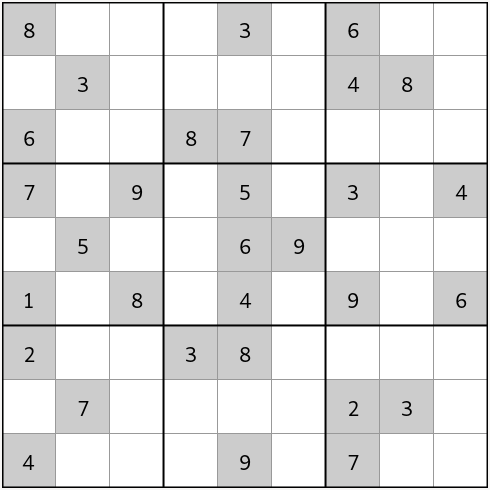
\includegraphics[width=.5\textwidth]{sudoku}
%%\\
%\mbox{} \hfill {\tiny The Book of Bunny Suicides \copyright Andy Riley}
\end{center}
%% \vfill \vfill
%\mbox{}

\newpage

% ABSCHLUSSKLAUSUR ;;;

\begin{klaufg}{8}{Reproduktion}
  Sei $K$ ein K"orper, und sei $F \colon M(2 \times 2;K) \to M(2
  \times 2;K)$ der durch $F(A) = \transpose A$ gegebene
  Endomorphismus.

  Bestimmen Sie $\det F$, $P_F$, $M_F$, Eigenwerte, Eigenr"aume und
  entscheiden Sie, ob $F$ diagonalisierbar ist.
\end{klaufg}

\pagebreak
\begin{klaufg}{4+4}{examples}

  \makebox[0pt][r]{($i$) }%
  Geben Sie Beispiele f"ur zwei Matrizen mit dem charakteristischen Polynom
  $(2+t)^2(3-t)$, sodass die eine diagonalisierbar ist und die andere
  nicht.

  (Begr"unden Sie {\bfseries\sffamily kurz}, dass Ihre Beispiele die
  geforderten Eigenschaften haben.)
  \pagebreak
  
  \makebox[0pt][r]{($ii$) }%
  Geben Sie ein Beispiel einer $11 \times 11$ Matrix $B$, so dass
  $\dim \ker B = 4$, $\dim \ker B^2 = 8$, $\dim \ker B^3 = 10$,
  $\dim \ker B^4 = 11$.
  
  (Begr"unden Sie {\bfseries\sffamily kurz}, dass Ihr Beispiel die
  geforderten Eigenschaften hat.)
\end{klaufg}

\pagebreak
\begin{klaufg}{4+4}{einfacher Beweis}
  \makebox[0pt][r]{($i$) }%
Sei $A \in M(n \times n; \R)$ symmetrisch positiv
definit. Zeigen Sie, dass $\det A$ das Produkt der Eigenwerte
(mit Vielfachheiten) von $A$ ist.
\vfill

\makebox[0pt][r]{($ii$) }%
Geben Sie ein Beispiel, das zeigt, dass man die Voraussetzung, dass
$A$ symmetrisch positiv definit ist, nicht ersatzlos streichen kann.

(Begr"unden Sie {\bfseries\sffamily kurz}, dass Ihre Matrix ein
geeignetes Beispiel ist.)
\vfill

\end{klaufg}

\pagebreak
\begin{klaufg}{8}{einfache Modellierung/Beweis}
  Sei $V$ ein unit"arer Vektorraum, und seien $F,G \in
  \Hom(V,V)$ selbstadjungiert. Zeigen Sie, dass $FG$ genau dann
  selbstadjungiert ist, wenn $FG=GF$.
\end{klaufg}
 
\pagebreak
{\bfseries Nur eine der Aufgaben 5 \& 6 wird gewertet.}
\bigskip
\bigskip

\begin{klaufg}{8}{hard1}
   Sei $V$ ein $n$-dimensionaler Vektorraum, und sei $F \in
   \operatorname{Hom}(V,V)$ invertierbar mit charakteristischem
   Polynom $$P_F(t) = (-1)^n t^n + a_{n-1} t^{n-1} + \cdots + a_1 t +
   a_0 .$$

   Zeigen Sie, dass es ein Polynom $g \in K[t]$ gibt mit $g(F)= F^{-1}$.
   \medskip

   \underline{\emph{Hinweis:}} Cayley--Hamilton; $a_0 \neq 0$.  
\end{klaufg}

\pagebreak
{\bfseries Nur eine der Aufgaben 5 \& 6 wird gewertet.}
\bigskip
\bigskip

\begin{klaufg}{8}{hard2}
  Es sei $U$ eine unit"are Matrix. Dann wissen wir, 
  \begin{enumerate}
  \item dass es eine unit"are Matrix $\tilde{U}$ und eine Diagonalmatrix
    $D$ gibt, sodass
    \[ U = \tilde{U} D \tilde{U}^{-1}\,, \text{ sowie}
    \]
  \item dass
    es unit"are Matrizen $\widehat{U}$ und $\widehat{V}$ und eine
    Diagonalmatrix $\Sigma$ gibt, sodass
    \[ U = \widehat{U} \Sigma \widehat{V}^*
    \]
    eine Singul"arwertzerlegung von $U$ ist.
  \end{enumerate}
  Dabei sind die Diagonaleintr"age von $\Sigma$ und von $D$ jeweils
  bis auf ihre Reihenfolge eindeutig durch $U$ bestimmt. (All das
  brauchen Sie {\bfseries nicht} zu zeigen.)

  Beweisen Sie oder widerlegen Sie mit konkretem Beispiel: $\Sigma$ und
  $D$ haben notwendigerweise dieselben Diagonaleintr"age.
\end{klaufg}

\end{document}


\pagebreak
NACHKLAUSUR ;;;

\begin{klaufg}{4+4}{Reproduktion}
  Sei $K$ ein K"orper, und sei $F \colon K[t]_{\le3} \to K[t]_{\le3}$
  der durch $F(f) = f(1)\,t^2$ gegebene Endomorphismus.

  Berechne $\det F$, $P_F$, Eigenwerte, Eigenr"aume und entscheide, ob
  $F$ diagonalisierbar ist.
  \end{klaufg}

\pagebreak
\begin{klaufg}{4+4}{examples}

  \makebox[0pt][r]{($i$) }%

  Geben Sie Beispiele von ...

  (Begr"unden Sie {\bfseries\sffamily kurz}, dass Ihr Beispiel die
  geforderten Eigenschaften hat.)
  \pagebreak
  
  \makebox[0pt][r]{($ii$) }%
    Geben Sie Beispiele von ...
  
  (Begr"unden Sie {\bfseries\sffamily kurz}, dass Ihr Beispiel die
  geforderten Eigenschaften hat.)

\end{klaufg}

\pagebreak
\begin{klaufg}{8}{einfacher Beweis}
  Sei $V$ ein endlichdimensionaler Vektorraum "uber dem K"orper $K$
  und seien $F,G \in \Hom(V,V)$ simultan diagonalisierbar. Das hei"st,
  es gibt eine Basis von $V$, die Eigenvektoren von $F$ und von $G$
  sind.

  Zeige, dass $FG=GF$.
\end{klaufg}

\pagebreak
\begin{klaufg}{8}{einfache Modellierung/Beweis}
  Sei $V$ ein $n$-dimensionaler Vektorraum, und sei $F \in \Hom(V,V)$
  ein Endomorphismus vom Rang eins.
  Zeigen Sie, dass entweder $F^2=0$ oder $F$ ist diagonalisierbar
  (aber nicht beides).

  \underline{\emph{Hinweis:}} $\dim(\im F \cap \ker F) = ?$
\end{klaufg}

\pagebreak
{\bfseries Nur eine der Aufgaben 5 \& 6 wird gewertet.}
\bigskip
\bigskip

\begin{klaufg}{8}{hard1}

\end{klaufg}

\pagebreak
{\bfseries Nur eine der Aufgaben 5 \& 6 wird gewertet.}
\bigskip
\bigskip

\begin{klaufg}{8}{hard2}
Sei $V$ ein endlichdimensionaler $\C$-Vektorraum, und sei $F \in
\Hom(V,V)$ so dass $F^6 = \id_V$.

Zeigen Sie, dass es ein Skalarprodukt $\langle .,. \rangle$ auf $V$
gibt, so dass $F$ unit"ar ist.  
\end{klaufg}



\end{document}





%%% Local Variables:
%%% mode: latex
%%% End:
